\documentclass[twoside,twocolumn]{article}

\usepackage{blindtext} % Package to generate dummy text throughout this template 
\usepackage{graphicx}
\usepackage[sc]{mathpazo} % Use the Palatino font
\usepackage[T1]{fontenc} % Use 8-bit encoding that has 256 glyphs
\linespread{1.05} % Line spacing - Palatino needs more space between lines
\usepackage{microtype} % Slightly tweak font spacing for aesthetics

\usepackage[english]{babel} % Language hyphenation and typographical rules

\usepackage[hmarginratio=1:1,top=32mm,columnsep=20pt]{geometry} % Document margins
\usepackage[hang, small,labelfont=bf,up,textfont=it,up]{caption} % Custom captions under/above floats in tables or figures
\usepackage{booktabs} % Horizontal rules in tables

\usepackage{lettrine} % The lettrine is the first enlarged letter at the beginning of the text

\usepackage{enumitem} % Customized lists
\setlist[itemize]{noitemsep} % Make itemize lists more compact

\usepackage{abstract} % Allows abstract customization
\renewcommand{\abstractnamefont}{\normalfont\bfseries} % Set the "Abstract" text to bold
\renewcommand{\abstracttextfont}{\normalfont\small\itshape} % Set the abstract itself to small italic text

\usepackage{titlesec} % Allows customization of titles
\renewcommand\thesection{\Roman{section}} % Roman numerals for the sections
\renewcommand\thesubsection{\roman{subsection}} % roman numerals for subsections
\titleformat{\section}[block]{\large\scshape\centering}{\thesection.}{1em}{} % Change the look of the section titles
\titleformat{\subsection}[block]{\large}{\thesubsection.}{1em}{} % Change the look of the section titles

\usepackage{fancyhdr} % Headers and footers
\pagestyle{fancy} % All pages have headers and footers
\fancyhead{} % Blank out the default header
\fancyfoot{} % Blank out the default footer
\fancyhead[C]{El Aseguramiento de la Calidad de Software  $\bullet$ Mayo 2019 $\bullet$ } % Custom header text
\fancyfoot[RO,LE]{\thepage} % Custom footer text

\usepackage{titling} % Customizing the title section

\usepackage{hyperref} % For hyperlinks in the PDF

%----------------------------------------------------------------------------------------
%	TITLE SECTION
%----------------------------------------------------------------------------------------

\setlength{\droptitle}{-4\baselineskip} % Move the title up

\pretitle{\begin{center}\Huge\bfseries} % Article title formatting
\posttitle{\end{center}} % Article title closing formatting
\title{ Cobol vs Ruby} % Article title
\author{Yaneth Aquino,,Bianca Chura ,Adnner Esperilla y Johanna Torres}
\date{\today} % Leave empty to omit a date
\renewcommand{\maketitlehookd}{%
\begin{abstract}
\noindent La comparación de lenguajes de programación es un tema común de discusión entre los ingenieros de software.
Pocos lenguajes son lo suficientemente populares como para que sean utilizados por más de unas pocas personas o que encuentren su nicho en la investigación o la educación;Pero los programadores profesionales pueden utilizar fácilmente docenas de idiomas diferentes durante su carrera.Se implementan cada año con el fin de mantenerse al día con la programación cambiante
paradigmas, evolución del hardware, etc.
\end{abstract}
}

%----------------------------------------------------------------------------------------

\begin{document}

% Print the title
\maketitle

%----------------------------------------------------------------------------------------
%	ARTICLE CONTENTS
%----------------------------------------------------------------------------------------

\section{Introduccion}

\lettrine[nindent=0em,lines=3]{L}os primeros lenguajes de programación de alto nivel fueron diseñados durante la década de 1950. Desde entonces, la programación
idiomas han sido un área de estudio fascinante y productiva . Miles de programación diferente
se han creado lenguajes, principalmente en el campo de la informática, y cada año se han creado muchos más; son
diseñados, especificados e implementados con el propósito de estar al día con la evolución de la programación
paradigmas (por ejemplo, imperativos, orientados a objetos, orientados a aspectos, reflexivos y funcionales, por nombrar algunos).
Mientras que algunos lenguajes de programación gozan de popularidad en todo el mundo y se utilizan comúnmente para desarrollar grandes,
aplicaciones de nivel empresarial (por ejemplo, C, C++, C, Java, PHP o Perl); otros sólo son utilizados por un número menor de
personas o están más orientados a la academia para la investigación y la educación (por ejemplo, OCaml, Haskell, Scheme, OZ, o
Scala).

%------------------------------------------------
\section{Objetivos}
\begin{itemize}
\item Establecer diferencias entre Cobol y ruby ,en las paradigmas de programacion.
\end{itemize}
%------------------------------------------------
\section{Desarrollo}
\subsection{COBOL}
\begin{itemize}
\item Es uno de los lenguajes de programación más antiguos (creado en 1959). Ha dominado la aplicación de software
desarrollo durante décadas y sigue siendo uno de los lenguajes de programación utilizados hoy en día en el software de negocios.
COBOL presenta diferentes ventajas, como simplicidad, portabilidad y
mantenimiento, también COBOL se considera muy poderoso en el procesamiento de datos masivos para las empresas Aplicaciones. COBOL ha sufrido varias mejoras (revisiones de 1968, 1974, 1985 y 2002) con el fin de ponerse al día con las nuevas tendencias de programación. La última encarnación de COBOL admite características orientadas a objetos
(todavía no hay ningún compilador compatible disponible) y también mantiene la compatibilidad con versiones anteriores.
\begin{center}
	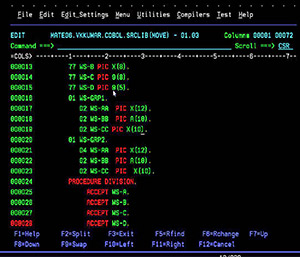
\includegraphics[width=7cm]{./Imagenes/3} 
	\end{center}
\subsection{Ruby}
\end{itemize}
Ruby es un lenguaje de programación dinámico, reflexivo y orientado a objetos de propósito general que combina sintaxis
inspirado por Perl con características similares a Smalltalk. Ruby se originó en Japón a mediados de la década de 1990 y fue
desarrollado y diseñado por Yukihiro "Matz" Matsumoto. Ruby es un lenguaje de programación puro orientado a objetos
con una sintaxis súper limpia que hace que la programación sea elegante y divertida. Ruby combina con éxito Smalltalk's
elegancia conceptual, la facilidad de uso y aprendizaje de Python, y el pragmatismo de Perl. Ruby ha comenzado a convertirse en
popular en todo el mundo en los últimos años como más libros en inglés y documentación se han convertido en
Disponible. Ruby soporta múltiples paradigmas de programación, incluyendo funcionales, orientados a objetos, imperativos,
y reflexivo. También cuenta con un sistema de tipo dinámico y gestión automática de la memoria
\begin{center}
	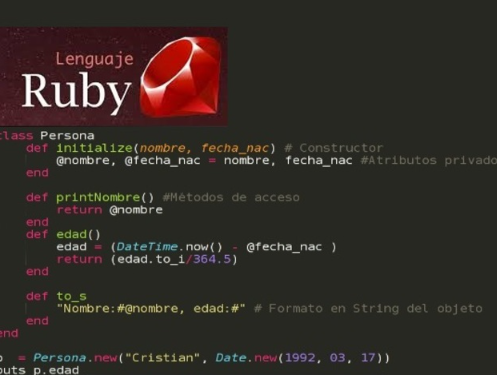
\includegraphics[width=5cm]{./Imagenes/2} 
	\end{center}
\subsection{Diferencia entre Cobol vs Rubi}
\begin{itemize}
\item COBOL
\\ \textbf{- Es un lenguaje prototípico AspectCOBOL para diseñar una extensión a COBOL para programación orientada a aspectos.}
\\ \textbf{- COBOL no puede hacer programación funcional.}
\\ \textbf{- COBOL es principalmente un lenguaje imperativo. }
\\ \textbf{- Muy conocido en secuencias de comandos por lotes, COBOL puede automatizar las tareas llamando a programas externos
como el controlador de la base de datos.}
\\ \textbf{-Generalmente los programas COBOL se ejecutan a través de
la línea de comandos, pero hay algunas herramientas
disponibles para crear interfaces gráficas (que
podría utilizarse para la creación de prototipos de interfaz de usuario).}
\item RUBY
\\ \textbf{- Ruby también cuenta con algunas extensiones:
AspectR-Fork y Aquarium siendo los más
popular y generalizada.}
\\ \textbf{-Los bloques, procs y lambdas de Ruby prestan
a sí mismos muy bien a una programación funcional
Estilo.
- Ruby carece de dos aspectos importantes para
programación funcional (coincidencia de patrones y
evaluación diferida), pero sus instalaciones, como
bloques, lambdas, y el hecho de que todo
se evalúa como una expresión que admite un
estilo de programación funcional
.}
\\ \textbf{-Los bloques, procs y lambdas de Ruby prestan
a sí mismos muy bien a una programación funcional
Estilo.
- Ruby carece de dos aspectos importantes para
programación funcional (coincidencia de patrones y
evaluación diferida), pero sus instalaciones, como
bloques, lambdas, y el hecho de que todo
se evalúa como una expresión que admite un
estilo de programación funcional
.}
\\ \textbf{-  Hay algunas opciones para ejecutar Batch
puestos de trabajo en Ruby, y también en los ferrocarriles
Marco de referencia. El módulo
ActiveRecord::Batches::ClassMethods permite
procesamiento de un gran número de registros y deportes
dos métodos principales para hacer scripting por lotes}
\\ \textbf{- Existen varias bibliotecas para permitir que Ruby
interacción gráfica del usuario (GUI).
}
\end{itemize}

\section{Conclusiones}
Es importante tomar decisiones tecnológicas en el momento adecuado y por las razones correctas. Buen negocio
las decisiones proporcionan a las buenas personas las herramientas de apoyo adecuadas para que puedan producir buenos productos.
Cuando se trata de desarrollo de software, lidiar con problemas de lenguaje difíciles de frente es una
requisito para el gerente visionario de hoy. Cuando se combina con otra ingeniería de software
consideraciones, una buena decisión de lenguaje puede apoyar el desarrollo de software rentable
sistemas que, a su vez, proporcionan un soporte empresarial valioso y confiable.


%---------------------------------------------------------------------------------------- 
%----------------------------------------------------------------------------------------
%	REFERENCE LIST
%----------------------------------------------------------------------------------------

\begin{thebibliography}{99} % Bibliography - this is intentionally simple in this template

 
\newblock Al-Qahtani, S. S., Pietrzynski, P., Guzman, L. F., Arif, R., & Tevoedjre, A. (2010). Comparing selected criteria of programming languages java, php, c++, perl, haskell, aspectj, ruby, cobol, bash scripts and scheme revision 1.0-a team cplgroup comp6411-s10 term report. arXiv preprint arXiv:1008.3434.
\end{thebibliography}

%----------------------------------------------------------------------------------------

\end{document}
